\documentclass{article}

\RequirePackage{luatex85}
\usepackage{fontspec}
\usepackage[all]{xy}

\usepackage{fancyhdr}
\usepackage{extramarks}
\usepackage{amsthm,amsmath,amssymb,physics}
\usepackage{tikz}
\usepackage{float}
\usepackage{subcaption}
\usepackage{graphicx}
\usepackage{siunitx}
\usepackage{minted}
\usemintedstyle{vs}

% ====================
% Basic Document Settings
%

\usepackage{pgfplots}

\topmargin=-0.45in
\evensidemargin=0in
\oddsidemargin=0in
\textwidth=6.5in
\textheight=9.0in
\headsep=0.25in

\linespread{1.1}

\pagestyle{fancy}
\lhead{\hmwkAuthorName}
\chead{\hmwkClass : \hmwkTitle}
\rhead{\firstxmark}
\lfoot{\lastxmark}
\cfoot{\thepage}

\renewcommand\headrulewidth{0.4pt}
\renewcommand\footrulewidth{0.4pt}

\setlength\parindent{0pt}

%
% Create Problem Sections
%

\newcommand{\enterProblemHeader}[1]{
    \nobreak\extramarks{}{Problem \arabic{#1} continued on next page\ldots}\nobreak{}
    \nobreak\extramarks{Problem \arabic{#1} (continued)}{Problem \arabic{#1} continued on next page\ldots}\nobreak{}
}

\newcommand{\exitProblemHeader}[1]{
    \nobreak\extramarks{Problem \arabic{#1} (continued)}{Problem \arabic{#1} continued on next page\ldots}\nobreak{}
    \stepcounter{#1}
    \nobreak\extramarks{Problem \arabic{#1}}{}\nobreak{}
}

\setcounter{secnumdepth}{0}
\newcounter{partCounter}
\newcounter{homeworkProblemCounter}
\setcounter{homeworkProblemCounter}{1}
\nobreak\extramarks{Problem \arabic{homeworkProblemCounter}}{}\nobreak{}

%
% Homework Problem Environment
%
% This environment takes an optional argument. When given, it will adjust the
% problem counter. This is useful for when the problems given for your
% assignment aren't sequential. See the last 3 problems of this template for an
% example.
%
\newenvironment{homeworkProblem}[1][-1]{
    \ifnum#1>0
        \setcounter{homeworkProblemCounter}{#1}
    \fi

    \section{Problem \arabic{homeworkProblemCounter}}
    \setcounter{partCounter}{1}
    \enterProblemHeader{homeworkProblemCounter}
}{
    \exitProblemHeader{homeworkProblemCounter}
}


\newcommand{\hmwkTitle}{Homework\ \#6}
\newcommand{\hmwkDueDate}{11 June, 2020}
\newcommand{\hmwkClass}{CS364/AM792}
\newcommand{\hmwkAuthorName}{\textbf{Unathi K. Skosana}}

% Title Page

\title{
    \vspace{2in}
    \textmd{\textbf{\hmwkClass:\ \hmwkTitle}}\\
    \normalsize\vspace{0.1in}\small{Due\ on\ \hmwkDueDate\ at 23:59pm}\\
    \vspace{3in}
}

\author{\hmwkAuthorName}
\date{}

\renewcommand{\part}[1]{\textbf{\large Part \Alph{partCounter}}\stepcounter{partCounter}\\}

% Alias for the Solution section header
\newcommand{\solution}{\textbf{\large Solution}}

\begin{document}

\maketitle

\pagebreak

\begin{homeworkProblem}
  I have chosen the Keras deep learning API. Keras is built on top of popular
  machine learning library by Google, TensorFlow. According to Keras' about page,
  Keras is an infrastructure layer for differentiable programming, with the
  ability to efficiently compute the gradient of arbitrary differentiable
  expressions and low-level tensor operations on CPU, GPU or TPU. The reason for
  choosing \mintinline{python}{Keras} was because of it's
  popularity in the scientific python community, making it easier to find
  learning resources on the internet. The \mintinline{python}{TensorFlow}
  and \mintinline{python}{Keras} packages can be easily installed to a
  python virtual environment via \mintinline{python}{pip}.
\end{homeworkProblem}

\pagebreak

\begin{homeworkProblem}
  \textbf{(a)}
  Here the images from the previous assignment were resized to $224\times224$,
  and loaded onto a numpy array with the following code snippet.

  \begin{minted}{python}
    ## Building labels and training data
    train_data = []
    train_labels = []

    classes = ["Coast", "Forest", "Highway", "Kitchen",\
                    "Mountain", "Office", "Store", "Street", "Suburb"]

    for cl in classes:
      folder_path = os.path.join("../assets/assignment-6/dataset/train", cl)
      for fname in os.listdir(folder_path):
        fpath = os.path.join(folder_path, fname)
        im = io.imread(fpath)
        im_resized = transform.resize(im, (224, 224) , anti_aliasing=True)
        im_arr = img_to_array(im_resized)
        train_data.append(im_arr)
        train_labels.append(classes.index(cl))

    train_data = np.array(train_data)
    train_labels = np.array(train_labels)
  \end{minted}

\textbf{(b)}
\\
\\

The three convolutional stages consisted of a convolutional layer of kernel
size $2 \times 2$ with the layer sizes progressively increasing from $16$ to
$64$. Similarly, the max pooling layer was of size $2 \times 2$. These parameters
were taken from one of the code examples of Keras (Keras 2020) titled
'Image classification from scratch'. The model was trained with
\mintinline{python}{SGD}
for a mini batch size of $16$ and a learning rate of $0.005$ for $20$ epochs.
This yielded an accuracy of $66\%$ on the testing set. \\ \\

\textbf{(c)}
\\
\\

Using Keras' \mintinline{python}{ImageDataGenerator} we can augment some
of the training set images to randomly flip left-right so as to increase the
sample size. Furthermore a dropout of $50\%$ was added just before the final
stage of the model. In the same values for the learning rate, batch size and
number of epochs, which yielded an accuracy of roughly $73\%$. \\ \\

\pagebreak

\textbf{(d)}
\\
\\
The top-$1$ accuracy is just same as the test accuracy and the top-$3$ accuracy
for this model was $93.6\%$. The confusion matrix is given below

  \begin{align*}
    M_\mathcal{C} = \begin{bmatrix}
      187 & 2 & 44 & 9 & 8 & 8 & 0 & 0 & 2 \\
      4 & 187 & 0 & 4 & 15 & 3 & 10 & 5 & 0 \\
      10 & 4 & 114 & 15 & 2 & 4 & 2 & 7 & 2 \\
      0 & 0 & 0 & 82 & 0 & 16 & 8 & 1 & 3 \\
      33 & 27 & 28 & 28 & 125 & 16 & 3 & 12 & 2 \\
      0 & 0 & 0 & 12 & 0 & 103 & 0 & 0 & 0 \\
      0 & 3 & 0 & 21 & 0 & 10 & 162 & 11 & 8 \\
      0 & 2 & 2 & 10 & 1 & 7 & 12 & 153 & 5 \\
      0 & 0 & 2 & 10 & 0 & 5 & 5 & 4 & 115 \\
    \end{bmatrix}
  \end{align*}

  Here are a few samples of correctly classified test images.

  \begin{figure}[H]
    \begin{subfigure}{0.5\textwidth}
      \centering
      \caption{Coast scene correctly identified}
      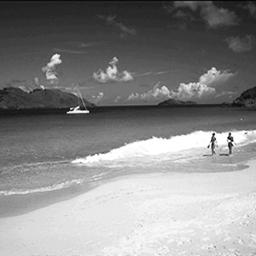
\includegraphics[width=.5\linewidth]{./images/own/coast_match_1.jpg}
    \end{subfigure}%
    \begin{subfigure}{0.5\textwidth}
      \centering
      \caption{Kitchen scene correctly identified}
      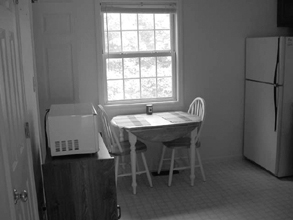
\includegraphics[width=.5\linewidth]{./images/own/kitche_match_2.jpg}
    \end{subfigure}
    \begin{subfigure}{0.5\textwidth}
      \centering
      \caption{Forest scene correctly identified}
      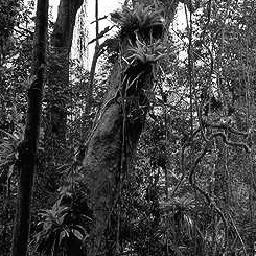
\includegraphics[width=.5\linewidth]{./images/own/forest_match_3.jpg}
    \end{subfigure}%
    \begin{subfigure}{0.5\textwidth}
      \centering
      \caption{Mountain scene correctly identified}
      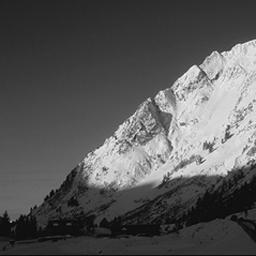
\includegraphics[width=.5\linewidth]{./images/own/mountain_match_4.jpg}
    \end{subfigure}
    \begin{subfigure}{0.5\textwidth}
      \centering
      \caption{Forest scene identified}
      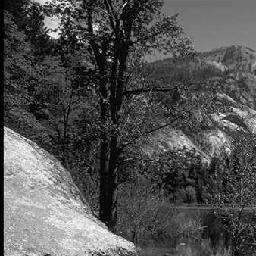
\includegraphics[width=.5\linewidth]{./images/own/forest_match_5.jpg}
    \end{subfigure}%
  \end{figure}

  \pagebreak

  Here are a few samples of incorrectly classified test images.

  \begin{figure}[H]
    \begin{subfigure}{0.5\textwidth}
      \centering
      \caption{Mountain scene incorrectly identified as a coast scene}
      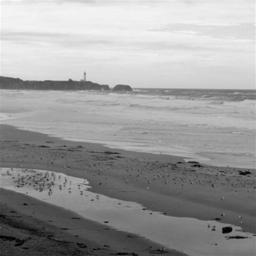
\includegraphics[width=.5\linewidth]{./images/own/coast_mountain_1.jpg}
    \end{subfigure}%
    \begin{subfigure}{0.5\textwidth}
      \centering
      \caption{Coast scene incorrectly identified as a mountain scene}
      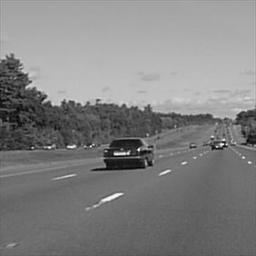
\includegraphics[width=.5\linewidth]{./images/own/highway_coast_1.jpg}
    \end{subfigure}
    \begin{subfigure}{0.5\textwidth}
      \centering
      \caption{Office scene incorrectly identified as a office scene}
      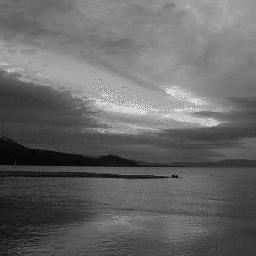
\includegraphics[width=.5\linewidth]{./images/own/coast_office_1.jpg}
    \end{subfigure}%
    \begin{subfigure}{0.5\textwidth}
      \centering
      \caption{Kitchen scene incorrectly identified as mountain scene}
      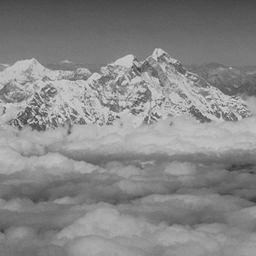
\includegraphics[width=.5\linewidth]{./images/own/moutain_kitchen_1.jpg}
    \end{subfigure}
    \begin{subfigure}{0.5\textwidth}
      \centering
      \caption{Highway scene incorrectly identified as mountain scene}
      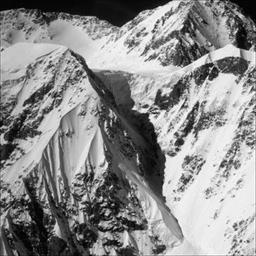
\includegraphics[width=.5\linewidth]{./images/own/moutain_highway_1.jpg}
    \end{subfigure}%
  \end{figure}
\end{homeworkProblem}

\pagebreak

\begin{homeworkProblem}
  \textbf{(a)}
  \\
  \\

  The model I choose for transfer learning was InceptionV3, primarily because of
  it's high top-$1$ accuracy, only second to Microsoft's ResNet, this plausibly due to the
  network being less deep than the latter. Google's InceptionV3 is mainly focused on
  computational cost (Google Cloud 2020), with ResNet focused on accuracy. However,
  the error rate of ResNet is not marginally better than InceptionV3's.
  So with the resources (inc. time) available to me at the time of writing prompt
  me to use InceptionV3. \\ \\

  \textbf{(b)}
  \\
  \\

  The input tensor was of shape $(224,224, 3)$, this was done by repeating the
  grayscale value of a pixel across the three channels, then appropriately
  converting these values to integer values. This data was then preprocessed by
  a helper function from Keras so that it lies in the range $[-1,1]$. Using the
  same values for the learning rate, batch size and number of epochs, after
  fitting the model, the model yielded $95\%$ accuracy on the test set. \\ \\


  \textbf{(c)}
  \\
  \\
  The top-$1$ accuracy is the same the test accuracy here as well. The top-$3$
  accuracy is an outstanding $99\%$ ! The confusion matrix is given below

  \begin{align}
    M_\mathcal{C} &= \begin{bmatrix}
      241 & 3 & 5 & 0 & 8 & 0 & 3 & 0 & 0\\
      1 & 210 & 2 & 0 & 8 & 0 & 5 & 0 & 2\\
      2 & 0 & 144 & 1 & 1 & 0 & 1 & 11 & 0\\
      0 & 0 & 0 & 100 & 0 & 8 & 2 & 0 & 0\\
      1 & 5 & 0 & 0 & 268 & 0 & 0 & 0 & 0\\
      0 & 0 & 0 & 2 & 0 & 113 & 0 & 0 & 0\\
      0 & 0 & 0 & 4 & 0 & 2 & 208 & 0 & 1\\
      0 & 0 & 4 & 0 & 0 & 0 & 4 & 181 & 3\\
      0 & 2 & 0 & 0 & 0 & 0 & 0 & 1 & 138\\
    \end{bmatrix}
  \end{align}

  \begin{figure}[H]
    \begin{subfigure}{0.5\textwidth}
      \centering
      \caption{Forest scene incorrectly identified as a mountain scene}
      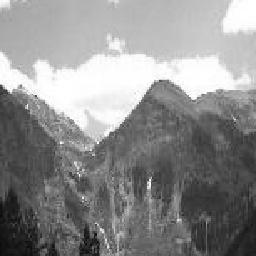
\includegraphics[width=.5\linewidth]{./images/incept/mountain_forest_1.jpg}
    \end{subfigure}%
    \begin{subfigure}{0.5\textwidth}
      \centering
      \caption{Mountain scene incorrectly identified as a coast scene}
      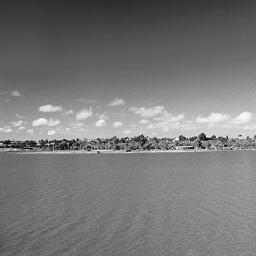
\includegraphics[width=.5\linewidth]{./images/incept/coast_mountain_1.jpg}
    \end{subfigure}
    \begin{subfigure}{0.5\textwidth}
      \centering
      \caption{Suburb scene incorrectly identified as a forest scene}
      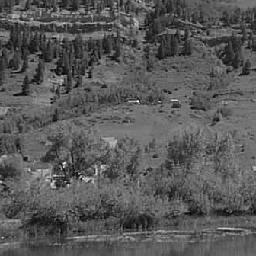
\includegraphics[width=.5\linewidth]{./images/incept/forest_suburb_1.jpg}
    \end{subfigure}%
    \begin{subfigure}{0.5\textwidth}
      \centering
      \caption{Street scene incorrectly identified as a highway scene}
      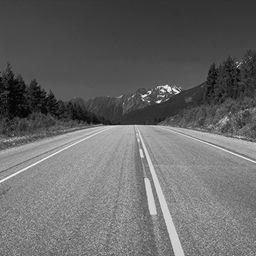
\includegraphics[width=.5\linewidth]{./images/incept/highway_street_1.jpg}
    \end{subfigure}
    \begin{subfigure}{0.5\textwidth}
      \centering
      \caption{Forest scene incorrectly identified as coast scene}
      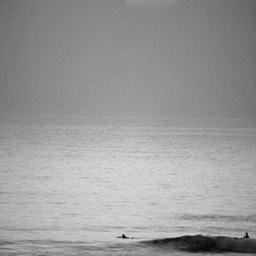
\includegraphics[width=.5\linewidth]{./images/incept/coast_forest_1.jpg}
    \end{subfigure}%
  \end{figure}

  \pagebreak
  Here are a few samples of correctly identified images.

  \begin{figure}[H]
    \begin{subfigure}{0.5\textwidth}
      \centering
      \caption{Coast scene correctly identified}
      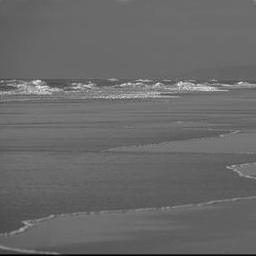
\includegraphics[width=.5\linewidth]{./images/incept/coast_match_1.jpg}
    \end{subfigure}%
    \begin{subfigure}{0.5\textwidth}
      \centering
      \caption{Store scene correctly identified}
      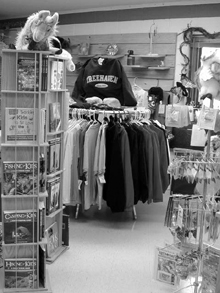
\includegraphics[width=.5\linewidth]{./images/incept/store_match_1.jpg}
    \end{subfigure}
    \begin{subfigure}{0.5\textwidth}
      \centering
      \caption{Store scene correctly identified}
      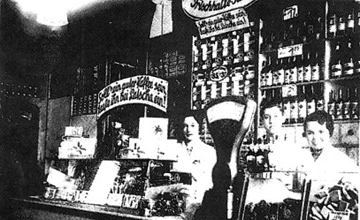
\includegraphics[width=.5\linewidth]{./images/incept/store_match_2.jpg}
    \end{subfigure}%
    \begin{subfigure}{0.5\textwidth}
      \centering
      \caption{Mountain scene correctly identified}
      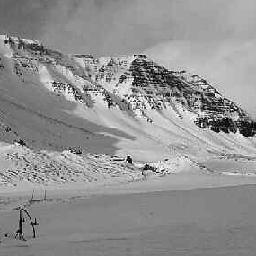
\includegraphics[width=.5\linewidth]{./images/incept/mountain_match_1.jpg}
    \end{subfigure}
    \begin{subfigure}{0.5\textwidth}
      \centering
      \caption{Street scene correctly identified}
      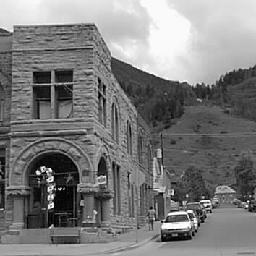
\includegraphics[width=.5\linewidth]{./images/incept/street_match_1.jpg}
    \end{subfigure}%
  \end{figure}

\end{homeworkProblem}



\section{References}
  Keras.io, \emph{Code examples}, viewed 11 June 2020,
  https://Keras.io/examples/ \\
  Google Cloud, \emph{Advanced Guide to Inception v3 on Cloud TPU}, viewed 11 June 2020, https://cloud.google.com/tpu/docs/inception-v3-advanced


\end{document}
